\documentclass[../Main/Knit.tex]{subfiles}

\section{Introduction}
 
\subsection{Mouse model of AD amyloidopathy: J20}
A mouse model of amyloidopathy, J20 overexpresses a mutant form human APP with two mutations identified by FAD, Indiana (V717F) and Swedish (K670N/M671L) mutations, directed by human platelet-growth-factor-beta promoter (PGRF-beta) with expression highest in the neocortex and hippocampus [Figure to show effects of mutations]. 
These mice exhibit defects in spatial memory and learning, with amyloid deposition by 5 – 7 moths, robust plaque formation by 8 – 10 months, and age-associated neuronal loss throughout the hippocampus. While J20 mouse closely resembles amyloidopathy development in human AD, insertion site of APP transgene has been shown to disrupt ZBTB20, a transcriptional repressor involved in hippocampal development.  

\subsection{Mouse model of AD tauopathy: rTg4510} 
Unlike with APP, there are currently no known mutations in MAPT linked to AD. Mouse models, such as rTG4510, that recapitulate AD tauopathy are therefore developed through harbouring missense mutations in MAPT that are associated with tauopathy in familial frontotemporal dementia (FTD). In the case with rTg4510, the human tau transgene carrying the P301L mutation is over-expressed under the calcium calmodulin kinase II promotor (CaMK2a) and is largely restricted to the forebrain (such as hippocampus and cortex). 
These mice also exhibit cognitive and behavioural impairments, with neurofibrillary tangles developing as early as 2 months, and associated neuronal and synaptic loss evident by 9 months. Starting from the neocortex and progressing rapidly to the hippocampus, the age-dependent spread of neuropathology in rTG4510 mouse closely reflects the spread of NFTs in human AD, as classified into Braak stages. However, it is important to note that the genomic integration of CAMK2a and MAPT transgene has been to have off-target effects with disruption in the endogenous mouse genes, including XXX. 
[Figure X: rTg4510 with image of why it is called regulatable due to the mouse line]


\newpage
\section{Methods}
As detailed in Chapter X, Pacific Biosciences Iso-Seq dataset was generated with whole transcriptome approach using high quality RNA from i) 12 mouse cortex (WT = 6, TG = 6) (Figure \ref{fig:isoseq_samples}). As a technological comparison and validation of the IsoSeq approach, a subset of samples were also sequenced on ONT (Figure \ref{fig:ONT_samples}). While both long-read sequencing approaches are superior to short-read RNA-Sequencing in the generation of full-length transcripts, there are major inherent batch biases due to the time-consuming and laborious protocol involved. The library preparation was standardised as much as possible, with the initial input of RNA for cDNA synthesis and the final library input for sequencing. However, due to the need for optimising each sample for library preparation and the rapid updates of sequencing chemistry throughout my PhD, each sample was effectively sequenced sequentially rather than as a batch [Figure X]. 

\begin{figure}[h]
	\includegraphics[page=2, width=1\linewidth,height=0.4\textheight]{Pictures/IsoSeq_Samples.png}
	\captionsetup{width=0.95\textwidth}
	\caption[Tg4510 WT and TG samples sequenced using Whole and Targeted Iso-Seq]%
	{\textbf{Tg4510 WT and TG samples sequenced using Whole and Targeted Iso-Seq}: 12 samples at baseline and final age timepoint (WT = 6, TG = 6, ages = 2 months, 8 months) were sequenced using Whole Iso-Seq (highlighted boxes) and an additional 12 samples (WT = 6, TG = 6, ages = 4 months and 6 months) were sequenced using Targeted Iso-Seq (outlined). Text on each mouse figure refer to sample names}
	\label{fig:isoseq_samples}
\end{figure}

\begin{figure}[h]
	\includegraphics[page=2, width=1\linewidth,height=0.4\textheight]{Pictures/ONT_Samples.png}
	\captionsetup{width=0.95\textwidth}
	\caption[Tg4510 WT and TG samples sequenced using Whole and Targeted ONT]%
	{\textbf{Tg4510 WT and TG samples sequenced using Whole and Targeted ONT}: A subset of samples were also sequenced as whole transcriptome on ONT (WT = 1, TG = 1, age  = 2 months, highlighted boxes) and targeted on ONT (WT = 7, TG = 11, outlined). Text on each mouse figure refer to sample names}
	\label{fig:ONT_samples}
\end{figure}



\newpage
\section{Results}

The mouse transcriptome of 12 pooled samples (WT and TG) was sequenced and analysed with the PacBio Sequel 1 platform for deep characterisation of full-length splice variants and identification of novel transcripts. 

Following library preparation and single-molecule real time sequencing (SMRT), a total of 371Gb (s.d = 4.35Gb, range = 22.5Gb - 38.74Gb) and 8,082,647 polymerase reads (s.d = 63,013 reads, range = 530,974 - 733,495 reads) were obtained (Table \ref{tab:run_output}). No significant difference was reported between WT and TG (n = 12 animals, two-tailed unpaired t-test, t(10) = -0.636, P = 0.539,  Figure \ref{fig:run_rin_corr}), and no significant correlation was observed between run yield and RIN across samples (n = 12 animals, Pearson's correlation, t = -0.98, df = 10, P = 0.350, Figure \ref{fig:run_output}). Yield across all the samples are within the range as would expected from SMRT Iso-Seq library.   

%Check no difference between lengths CCS read lengths i.e. equal representation of RNA molecules; to make sure that we have a fair representation of reads of the RNA transcripts --> comparison of CCS reads and representation of RNA molecules between different base pairs lengths between different sample sets --> if fair representation, then expect log-ratio of interested sample/compared sample = - (10^0 =1)

\
\begin{table}[h]
	\begin{tabularx}{1\textwidth}{cccccc}
		\toprule
		Sample & Age      & Phenotype & RIN & Total Bases (GB) & Unique Yield (GB) \\ \midrule
		K17    & 2 months & WT   & 9.2 & 29.56            & -                           \\
		K18    & 2 months & TG   & 8.8 & 31.1             & 1.21                        \\
		K23    & 8 months & WT   & 9.1 & 34.60            & 2.06                        \\
		K24    & 8 months & TG   & 9.2 & 34.61            & 2.09                        \\
		L22    & 8 months & TG   & 8.7 & 38.74            & 2.1                         \\
		M21    & 2 months & WT   & 9.2 & 30.45            & -                           \\
		O18    & 2 months & TG   & 8.9 & 22.53            & 1.56                        \\
		O23    & 8 months & WT   & 9   & 31.25            & -                           \\
		Q20    & 8 months & TG   & 8.6 & 33.16            & 2.27                        \\
		Q21    & 2 months & WT   & 9.2 & 24.52            & 2.27                        \\
		S18    & 2 months & TG   & 8.9 & 30.41            & 1.69                        \\
		S23     & 8 months & WT   & 9.1 & 30.28            & -                          \\ \bottomrule
	\end{tabularx}
	\caption[Run Yield Output from Whole Transcriptome Iso-Seq of Tg4510]%
	{Phenotypic information and Iso-seq run yield for each sample of Tg4510 sequenced using Whole Transcriptome approach}
	\label{tab:run_output}
\end{table}

\begin{figure}[h]
	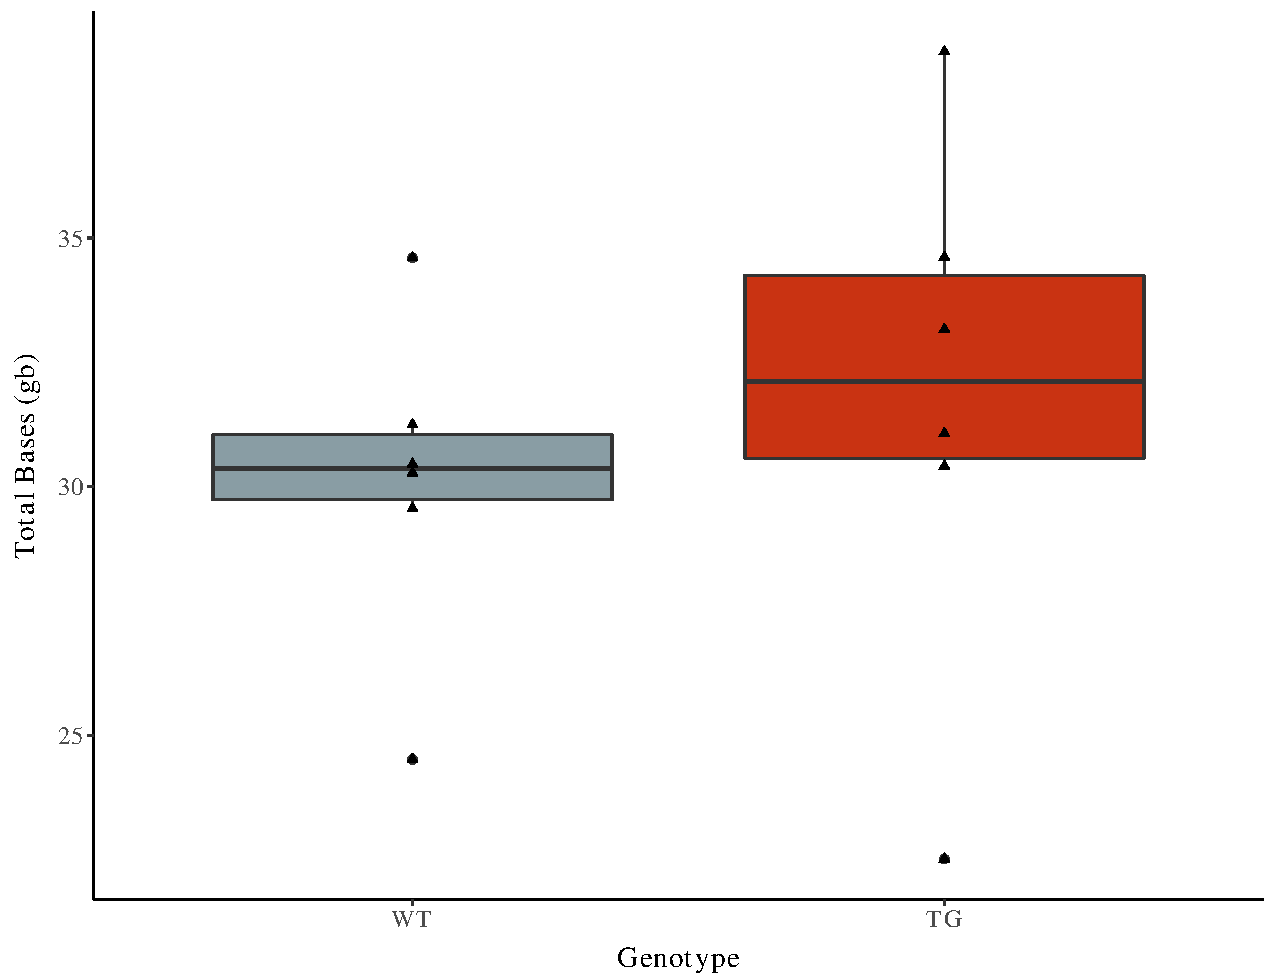
\includegraphics[page=1, width=1\linewidth,height=0.4\textheight]{Pictures/Tg4510_RunStats.pdf}
	\captionsetup{width=0.95\textwidth}
	\caption[Whole Transcriptome Iso-Seq run output in transgenic and wild type Tg4510 mouse model]%
	{\textbf{Whole Transcriptome Iso-Seq run output in transgenic and wild type Tg4510 mouse model}: No significant difference in run output was observed between WT and TG Tg4510 mice. Of note, two samples with $<$25Gb in WT and TG refer to earlier samples sequenced with a lower chemistry (Sequencing Primer v3; Sequel Binding Kit 2.1) and diffusion loading}
	\label{fig:run_output}
\end{figure}

\begin{figure}[h]
	\includegraphics[page=2, width=1\linewidth,height=0.4\textheight]{Pictures/Tg4510_RunStats.pdf}
	\captionsetup{width=0.95\textwidth}
	\caption[No significant correlation between RIN and Whole Transcriptome Iso-Seq run output]%
	{\textbf{No significant correlation between RIN and Whole Transcriptome Iso-Seq run output}: Samples with RIN $>$8 were selected for Whole Transcriptome Iso-Seq, with TG samples having distinctly lower RIN values than WT samples. However, no significant difference was observed for run output between WT and TG (Figure \ref{tab:run_output}) }
	\label{fig:run_rin_corr}
\end{figure}


\begin{landscape}
	\begin{table}[]
		\resizebox{1.5\textwidth}{!}{%
		\begin{tabular}{@{}cccccccccccccccccc@{}}
			\toprule
			\multirow{3}{*}{Sample} &
			\multirow{3}{*}{\begin{tabular}[c]{@{}c@{}}Polymerase\\ Reads\end{tabular}} &
			\multicolumn{6}{c}{Read   Length} &
			\multicolumn{3}{c}{Productivity} &
			\multicolumn{4}{c}{Control} &
			\multirow{3}{*}{\begin{tabular}[c]{@{}c@{}}Local\\  Base \\ Rate\end{tabular}} &
			\multicolumn{2}{c}{Template} \\ \cmidrule(lr){3-15} \cmidrule(l){17-18} 
			&
			&
			\multicolumn{2}{c|}{Polymerase} &
			\multicolumn{2}{c|}{Subread} &
			\multicolumn{2}{c|}{Insert} &
			\multicolumn{1}{c|}{\multirow{2}{*}{P0}} &
			\multicolumn{1}{c|}{\multirow{2}{*}{P1}} &
			\multicolumn{1}{c|}{\multirow{2}{*}{P2}} &
			\multicolumn{1}{c|}{\multirow{2}{*}{\begin{tabular}[c]{@{}c@{}}Total   \\ Reads\end{tabular}}} &
			\multicolumn{1}{c|}{\multirow{2}{*}{\begin{tabular}[c]{@{}c@{}}Pol RL  \\ Mean\end{tabular}}} &
			\multicolumn{2}{c|}{Concordance} &
			&
			\multicolumn{1}{c|}{\multirow{2}{*}{\begin{tabular}[c]{@{}c@{}}Adapter   \\ Dimer \\ (0-10bp)\end{tabular}}} &
			\multicolumn{1}{c|}{\multirow{2}{*}{\begin{tabular}[c]{@{}c@{}}Short\\  Insert\\  (11- 100bp)\end{tabular}}} \\ \cmidrule(lr){3-8} \cmidrule(lr){14-15}
			&
			&
			\multicolumn{1}{c|}{Mean} &
			\multicolumn{1}{c|}{N50} &
			\multicolumn{1}{c|}{Mean} &
			\multicolumn{1}{c|}{N50} &
			\multicolumn{1}{c|}{Mean} &
			\multicolumn{1}{c|}{N50} &
			\multicolumn{1}{c|}{} &
			\multicolumn{1}{c|}{} &
			\multicolumn{1}{c|}{} &
			\multicolumn{1}{c|}{} &
			\multicolumn{1}{c|}{} &
			\multicolumn{1}{c|}{Mean} &
			\multicolumn{1}{c|}{Mode} &
			&
			\multicolumn{1}{c|}{} &
			\multicolumn{1}{c|}{} \\ \midrule
			B21 &
			735598 &
			39971 &
			82100 &
			1531 &
			2125 &
			3162 &
			3896 &
			\begin{tabular}[c]{@{}c@{}}8.71\% \\ (87817)\end{tabular} &
			\begin{tabular}[c]{@{}c@{}}73.94\% \\ (745646)\end{tabular} &
			\begin{tabular}[c]{@{}c@{}}18.33\% \\ (184883)\end{tabular} &
			9940 &
			34144 &
			0.85 &
			0.89 &
			2.61 &
			0 &
			0 \\
			C20 &
			749931 &
			45670 &
			91153 &
			1426 &
			2066 &
			3204 &
			4075 &
			\begin{tabular}[c]{@{}c@{}}10.68\% \\ (107699)\end{tabular} &
			\begin{tabular}[c]{@{}c@{}}75.36\% \\ (759912)\end{tabular} &
			\begin{tabular}[c]{@{}c@{}}14.95\% \\ (150735)\end{tabular} &
			9910 &
			37019 &
			0.85 &
			0.89 &
			2.75 &
			0 &
			0 \\
			C21 &
			530395 &
			44208 &
			87750 &
			2258 &
			2794 &
			3358 &
			4250 &
			\begin{tabular}[c]{@{}c@{}}38.0\% \\ (387661)\end{tabular} &
			\begin{tabular}[c]{@{}c@{}}52.5\% \\ (535299)\end{tabular} &
			\begin{tabular}[c]{@{}c@{}}9.4\% \\ (96275)\end{tabular} &
			4880 &
			50690 &
			0.85 &
			0.85 &
			2.07 &
			0.00 &
			0.01 \\
			E18 &
			545,272 &
			41,036 &
			83,295 &
			2,467 &
			3,049 &
			3,588 &
			4,335 &
			\begin{tabular}[c]{@{}c@{}}38.88\% \\ (396026)\end{tabular} &
			\begin{tabular}[c]{@{}c@{}}53.61\% \\ (546027)\end{tabular} &
			\begin{tabular}[c]{@{}c@{}}7.58\% \\ (77181)\end{tabular} &
			722 &
			48,253 &
			0.85 &
			0.85 &
			2 &
			0 &
			0 \\
			K17 &
			673972 &
			43856 &
			90561 &
			1253 &
			2021 &
			3336 &
			4753 &
			\begin{tabular}[c]{@{}c@{}}10.55\% \\ (106,736)\end{tabular} &
			\begin{tabular}[c]{@{}c@{}}67.42\% \\ (681,794)\end{tabular} &
			\begin{tabular}[c]{@{}c@{}}22.73\% \\ (229,816)\end{tabular} &
			7036 &
			34651 &
			0.85 &
			0.89 &
			2.72 &
			0.08 &
			0.06 \\
			K18 &
			566086 &
			54892 &
			101220 &
			1256 &
			1775 &
			2863 &
			3661 &
			\begin{tabular}[c]{@{}c@{}}29.77\%\\ (299933)\end{tabular} &
			\begin{tabular}[c]{@{}c@{}}57.25\% \\ (576863)\end{tabular} &
			\begin{tabular}[c]{@{}c@{}}14.05\% \\ (141550)\end{tabular} &
			10707 &
			44640 &
			0.87 &
			0.89 &
			3.05 &
			0 &
			0 \\
			K23 &
			698178 &
			49563 &
			98801 &
			1697 &
			2670 &
			3779 &
			4779 &
			\begin{tabular}[c]{@{}c@{}}16.1\% \\ (164308)\end{tabular} &
			\begin{tabular}[c]{@{}c@{}}69.2\%  \\ (704197)\end{tabular} &
			\begin{tabular}[c]{@{}c@{}}14.7\%   \\ (149841)\end{tabular} &
			5951 &
			40498 &
			0.85 &
			0.89 &
			2.78 &
			0 &
			0 \\
			K24 &
			711015 &
			48675 &
			97024 &
			1714 &
			2487 &
			3834 &
			5018 &
			\begin{tabular}[c]{@{}c@{}}14.22\% \\ (144813)\end{tabular} &
			\begin{tabular}[c]{@{}c@{}}70.49\%\\  (717880)\end{tabular} &
			\begin{tabular}[c]{@{}c@{}}15.28\% \\ (155653)\end{tabular} &
			6762 &
			38363 &
			0.85 &
			0.87 &
			2.671 &
			0.01 &
			0.01 \\
			L22 &
			675283 &
			57370 &
			112630 &
			1869 &
			2867 &
			3903 &
			4793 &
			\begin{tabular}[c]{@{}c@{}}17.41\%\\ (175439 )\end{tabular} &
			\begin{tabular}[c]{@{}c@{}}68.08\%\\ (686007)\end{tabular} &
			\begin{tabular}[c]{@{}c@{}}15.58\% \\ (156900)\end{tabular} &
			10647 &
			44215 &
			0.86 &
			0.89 &
			2.96 &
			0.01 &
			0 \\
			M21 &
			660841 &
			46082 &
			91628 &
			2234 &
			2754 &
			3952 &
			4733 &
			\begin{tabular}[c]{@{}c@{}}16.6\%\\ (168567)\end{tabular} &
			\begin{tabular}[c]{@{}c@{}}65.9\%  \\ (671224)\end{tabular} &
			\begin{tabular}[c]{@{}c@{}}17.5\% \\  (178555)\end{tabular} &
			10301 &
			38690 &
			0.85 &
			0.87 &
			2.79 &
			0.01 &
			0.01 \\
			O18 &
			530974 &
			42423 &
			85331 &
			2609 &
			3146 &
			3443 &
			4082 &
			\begin{tabular}[c]{@{}c@{}}41.8\% \\  (426378\end{tabular} &
			\begin{tabular}[c]{@{}c@{}}52.6\%\\  (536435)\end{tabular} &
			\begin{tabular}[c]{@{}c@{}}5.5\% \\ (56422)\end{tabular} &
			5415 &
			49778 &
			0.86 &
			0.85 &
			2.05 &
			0 &
			0 \\
			O23 &
			730733 &
			42771 &
			89372 &
			1490 &
			2347 &
			3608 &
			4878 &
			\begin{tabular}[c]{@{}c@{}}9.37\% \\ (94536)\end{tabular} &
			\begin{tabular}[c]{@{}c@{}}73.33\% \\ (740184)\end{tabular} &
			\begin{tabular}[c]{@{}c@{}}18.19\% \\ (183626)\end{tabular} &
			8908 &
			34993 &
			0.85 &
			0.89 &
			2.56 &
			0.06 &
			0.04 \\
			Q20 &
			715206 &
			46360 &
			92519 &
			1,999 &
			2,926 &
			3,978 &
			4,954 &
			\begin{tabular}[c]{@{}c@{}}11.51\%\\  (117223)\end{tabular} &
			\begin{tabular}[c]{@{}c@{}}70.91\% \\ (722135)\end{tabular} &
			\begin{tabular}[c]{@{}c@{}}17.58\%\\  (178988)\end{tabular} &
			6855 &
			37990 &
			0.85 &
			0.87 &
			2.6 &
			0.01 &
			0.01 \\
			Q21 &
			733495 &
			33429 &
			70750 &
			2563 &
			3286 &
			3710 &
			4750 &
			\begin{tabular}[c]{@{}c@{}}15.9\% \\ (161679)\end{tabular} &
			\begin{tabular}[c]{@{}c@{}}72.1\%\\  (735250)\end{tabular} &
			\begin{tabular}[c]{@{}c@{}}12.0\% \\ (122305)\end{tabular} &
			1668 &
			44201 &
			0.85 &
			0.85 &
			1.99 &
			0.00 &
			0.01 \\
			S18 &
			682529 &
			44549 &
			90041 &
			1435 &
			2041 &
			3282 &
			4400 &
			\begin{tabular}[c]{@{}c@{}}11.98\%\\  (121,055)\end{tabular} &
			\begin{tabular}[c]{@{}c@{}}68.45\% \\ (691651)\end{tabular} &
			\begin{tabular}[c]{@{}c@{}}20.35\%\\  (205,640)\end{tabular} &
			7881 &
			36541 &
			0.86 &
			0.89 &
			2.85 &
			0.11 &
			0.07 \\
			S23 &
			704335 &
			42991 &
			89160 &
			1346 &
			2020 &
			3272 &
			4383 &
			\begin{tabular}[c]{@{}c@{}}7.02\%\\  (71074)\end{tabular} &
			\begin{tabular}[c]{@{}c@{}}70.18\% \\ (710471)\end{tabular} &
			\begin{tabular}[c]{@{}c@{}}23.39\% \\ (236801)\end{tabular} &
			6019 &
			35167 &
			0.85 &
			0.89 &
			2.57 &
			0.01 &
			0.01 \\ \bottomrule
		\end{tabular}%
	}
	\end{table}
\end{landscape}


\subsection{Bioinformatics output}
Following the established bioinformatics pipeline [Figure X], a total of XXX successful CCS reads were generated (n = 12 samples, s.d = , range =  XX - XX) and a total of XXX FLNC reads obtained, post trimming of barcodes with LIMA and clustering of transcripts with Iso-Seq3. As described in Section X, the FLNC reads from the same isoform were then clustered to generate a total XXX high-quality transcripts (n = 12 samples, s.d = , range = XX - XX) with accuracy $>$99\% and XX low-quality transcripts (n = 12 samples, s.d = , range = XX - XX). XX isoforms (XX\%) were longer than 500 bp, and XXX transcripts (XX\%) were longer than 1-kb. No difference was observed in number of FLNC reads and number of transcripts between WT and TG. 

The clustered transcripts have an average length of XXX nt, with the longest being XXX nt. "The apparent length limitation to 6kb is most likely a combined result of ineffective size selection and the limitation ofthe sequencing chemistry (P4-C2, Methods) used in this study"; what are the proportion of transcripts relative to genome in size? The length of clustered transcripts closely reflect size distribution of the input full-length reads. "Final transcripts include a large number of isoforms greater than 3 kb that are not accessible by simply using CCS reads."   

Further stringent clustering and SQANTI filtering, as detailed in Section X, produced an average XX of unique transcripts and XX of genes with no differences identified between WT and TG in both rTg4510 (n = 12, two-tailed unpaired t-test) and J20 (n = 4, two-tailed unpaired t-test). Supplementary Table X records the number of transcripts prior and post SQANTI filtering.



\subsection{Genome Mapping}
HQ-isoforms from the pooled dataset were aligned to mouse genome using Minimap2, and a total of XXX reads (XX\%) were mapped. Errors for substitution, insertion and deletion are X\%, X\% and X\% respectively. XX\% of transcripts (polished) could not be mapped to reference genome, thus representing genes that fall into gaps in the assembly (mouse genome should be quite updated though)


\begin{enumerate}
	\item Unmapped reads with no signficant mapping to the genome: 
	\item Multiple mapped reads showing multiple alignment
	\item Reads mapped to positive strand of the genome
	\item Reads mapped to negative strand of the genome
\end{enumerate}


\subsection{Transcriptome annotation}
Post SQANTI filtering and removal of mono-exons, an average XX of unique transcripts were identified, with X\% coding and x\% non-coding. Corresponding with average transcript size in GENCODE and with bioanalyzer traces, the average length was XXX (range: XX, sd XX) with no difference reported between WT and TG in Tg4510 and J20 mouse models.  A wide range in the number of isoforms was identified per gene (XX – XX), with majority of genes characterised by more than $>$1 detectable isoform, and a notable proportion of genes characterised by >10 isoforms – difference between WT and TG?
[Saturation Curve] 

Mapped isoforms were divided into: 
\begin{enumerate}
	\item known isoforms from known genes
	\item novel isoforms from known genes 
	\item novel isoforms from novel genes 
\end{enumerate}
What percentage of FLNCs mapped?

\subsection{Exploring the PacBio transcriptome of the mouse reference genome}

\subsubsection{Protein Coding and non coding RNA genes and transcripts}
XX of protein coding transcripts from XX genes and XX non-coding transcripts from XX genes. Within the non-coding RNAs (ncRNAs), XX transcripts were longer than 200bp as classified as long noncoding RNAs. - Is there a difference in the number of exons between coding and non-coding transcripts i.e. single exon transcripts making up majority of non-coding RNAs. In \cite{Kuo2017}, and \cite{Chen2017}, observed a relatively higher proportion of mono-exon transcripts among non-coding RNAs than in human - likewse in mouse? rationale due to low sequencing depth and not able to detect many lowly expressed multiple exon RNA

\subsubsection{Nonsense mediated decay products} 

\subsubsection{Transcriptional Complexity}
Ratio of transcripts to genes? 
Assessment of alternative TSS, remove all genes with only one representative transcript as default only one TSS - XX (XX\%) had multiple TSS, high incidence likely due to a combination of library preparation error (resulting in wobble) and biological transcription start exons. Filtering transcripts with TSS caused by wobble, XX have multiple starting exons. 

Assessment of alternative TTS, similarly remove all genes with only one representative transcript. 

Assessment of retained introns and skipped exons in multi-transcript genes. 
Are there any alternative splicing differences between protein coding and lncRNA genes. 

Comparison of the PacBio transcriptome with public annotation - 


\subsection{Transcriptome abundance hierarchal between samples}
\textbf{Annotated genes}
Average XX of annotated genes (XX out of XX; range: XX, sd: XX) with an average length of XX was identified. No difference in number of annotated genes or distribution of isoforms in annotated genes was identified between Tg4510 and J20 mouse. Average XX full splice match isoforms were identified with no difference between Tg4510 and J20 mouse [Table X for breakdown]

Different splicing events annotated by SUPPA2. Reported differences in terms of numbers between types of splicing events in WT vs TG in Tg4510 and J20?

XX of known transcripts were identified to have intron retention; XX of known transcripts were identified to be fusion genes. XX of know transcripts identified to have non-sense-mediated decay. 


\subsection{Iso-Seq vs RNA-Seq} 
-	Correlation of IsoSeq TPM expression and RNASeq TPM expression 
-	What is the threshold of gene expression observed in Iso-Seq data vs RNA-Seq data (genes that are observed in RNA-Seq but not in Iso-Seq)
Isoform quantification using RNASeq 
-	Comparison of PacBio isoforms with short-read assembly from \cite{Gordon2015} \cite{Wang2016} by using short-read assembler such as Cufflinks and de-novo for construction of short reads, and considering locus that are only in evident in PacBio dataset and short-reads, less than 20\% of isoforms from PacBio dataset recapitulated

Unannotated novel genes with novel transcripts 
While majority of transcripts were annotated to known genes, X\% [range: XX, sd: XX] of transcripts were mapped to unannotated “novel” genes. These novel transcripts with mean length XXX bps (range: XX, std: XX) were identified uniformly across the genome/chromosome, with XX\% coding and XX\% non-coding. Majority (XX\%) of these novel genes had only 1 transcript, however, several novel genes were identified with 3 or more novel transcripts, highlighting the validity of these novel genes.
The validity of these novel genes is further supported by other resources. Using publicly available FANTOM5 Cap Analysis of Gene Expression (CAGE) that maps transcript, transcription factors, transcription promoters and enhancers (ref), majority of these novel genes (XX out of XX) in the mouse samples lie within 5kB of a cage peak. Junctions/Exons of these novel genes are also supported by aligned short-read RNA-Seq reads (XX out of XX). [Novel transcript abundance]
No reported differences in number of unannotated, novel transcripts were identified between Tg4510 and J20 mouse [XXX].

https://www.ncbi.nlm.nih.gov/pmc/articles/PMC6885035/ - Lorna’s paper on example of isoforms in their selective panel of genes that have differential quantification associated with AD. Good examples to check with transcriptome data to see if this is also observed in mouse (I.e. TAU3 increase) 

\subsection{Change in endogeneous expression}
%Check whether overexpression of human MAPT result in any unwanted, compensatory effects on equivalent mouse genes,as expression levels of mouse APP and MAPT should be slightly reduced, thereby suggesting no evidence that human transgene expression increase expression of directly-related mouse genes.
Supporting findings from \cite{Castanho2020}, human-specific MAPT sequences were only detected in CCS and FL reads from TG mice, confirming stable insertion and activation of MAPT transgene in TG mice. 

\subsection{ERCC}
One source of error from long-read sequencing can occur at reverse transcription, whereby a premature termination in reverse transcription enzyme can result in a full-length cDNA, that is mistaken for a true isoform. To measure the degree of this technical error, ERCC, with known start and end positions can be used as benchmark. As detailed in \cite{Karlsson2017}, most ERCC reads fell within +/- 5bp at both 5' and 3' ends, with 3' end slightly more accurate than 5' end. From \cite{Sharon2013}, drop in read length was observed for ERCC for molecules longer than 1.5kb (PacBio RSII). Interestingly, non-coding exon junctions were more variable than coding-exon junctions, suggesting that codon exon splicing has a stricter control with refined splice donor/acceptor sites (\citep{Karlsson2017}) 
Of note, however, that while ERCC has been used as a standard for RNA-Seq method validation, the longest molecule is only ~2kB, thus limiting is usage to validate longer molecules. Given that XX of RNA transcripts in human and mouse transcriptome are >2kB, there is a need for longer control sequences. 
 
\subsection{LncRNA}
lncRNA expression has been known to be more lowly expressed compared to protein-coding genes (\cite{Derrien2012}), and has been previously shown in other long-read studies (\cite{Tilgner2015})

\subsection{Isoform diversity}
Generally, higher gene expression, more isoforms observed (with linear increase); \citep{Karlsson2017}

\subsection{Splicing Events}
Single cell analysis (\cite{Karlsson2017}) noted that alternative TSS and TTS variation in the first exon representing more than 70\% of splicing events, with only around 30\% of 5' end transcripts located near annotated 5' (partially due to ongoing mRNA degradation, presence of unannotated alternative TSS, or strand invasion during reverse transcription resulting in template switching artefacts) and only around 70\% of 3'ends located at the annotated 3'ends (attributed to alternative polyadenylation sites in 3'UTR).

\subsection{Validation of novel isoforms}
- Profile of H3K4me3 enrichment, a chromatin signature of active promoters \citep{Qiao2020}
